\documentclass[12pt,a4paper]{article}
\usepackage[T2A]{fontenc}
\usepackage[utf8]{inputenc}
\usepackage[russian]{babel}
\usepackage{amsmath}
\usepackage{amssymb}
\usepackage{graphicx}
\usepackage{floatrow}
\usepackage{booktabs}
\usepackage{wrapfig}
\usepackage{lipsum}
\usepackage{subcaption}
\usepackage{fancyhdr}

\newcommand{\figref}[1]{(См. рис. \ref{#1})}
\newcommand{\secref}[1]{(См. раздел. \ref{#1})}

\newcommand{\e}[1]{\text{$\cdot10^{#1}$}}

\pagestyle{fancy}
\fancyhead{}
\fancyhead[L]{Работа 2.3.1}
\fancyhead[R]{}
\fancyfoot[C]{\thepage}

\author{\normalsize Выполнил: Дедков Денис, группа Б01-109 \\
	\normalsize 28.02.2022}
\date{}



\usepackage{float}
\restylefloat{table}
\title{
	\large Отчет о выполнении лабораторной работы 2.4.1 \\
	\Large Определение теплоты испарения жидкости \\ 
	
}


\begin{document}
	\maketitle
	\subsection*{Цель работы} 
	  1) измерение объемов форвакуумной и высоковакуумной частей установки; 2) определение скорости откачки системы в стационарном режиме, а также по ухудшению и по улучшению вакуума. 
	
	\subsection*{Оборудование и приборы} Экспериментальный стенд на основе компактного безмасляного высоковакуумного откачного поста Pfeiffer Vacuum серии
	HiCube 80 Eco с диафрагменным и турбомолекулярным насосами, вакуумметров Pfeiffer Vacuum серии DigiLine, и вакуумных быстроразъёмных
	компонентов. Блок управления (цифровой интерфейс RS-485).
	
	
\subsection*{Теоретическое введение}

В физике вакуумом называют состояние газа, при котором характерная длина свободного пробега молекул в газе $\lambda$ сравнима по порядку
величины с характерным линейным размером сосуда $d$, в котором газ
находится.

Основы процесса откачки и связанные с ним понятия рассмотрим
на примере простейшей вакуумной системы.

Предельное остаточное давление (предельный вакуум) $P_{\text{пр}}$ -- наименьшее давление газа, которое формируется в процессе откачки в рассматриваемом сечении вакуумпровода (рассматриваемой точке вакуумной системы). Обычно выделяют предельное давление в
камере или на входе в насос.

Наибольшее выпускное давление -- максимально допустимое давление газа на входе насоса.

\begin{figure}[h]
	\centering
	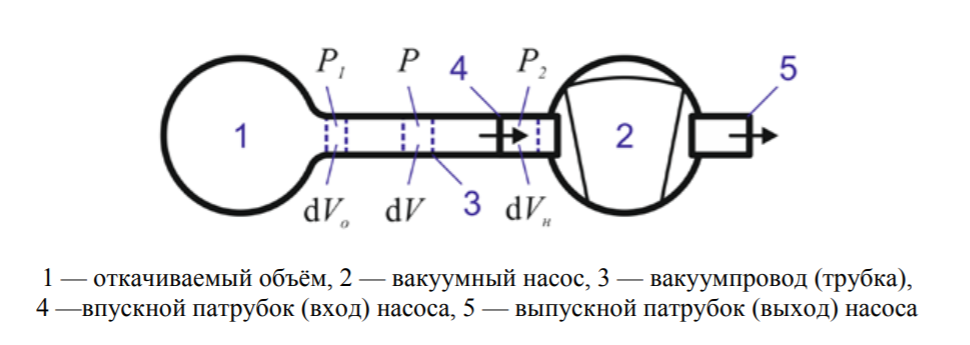
\includegraphics[width = 11 cm]{res/1}
	\caption{Простейшая вакуумная система}
	\label{fig:vac}
\end{figure}

Быстрота откачивающего действия (скорость откачки) вакуумной системы $S$ -- объем газа, проходящий через рассматриваемое сечение вакуумпровода в единицу времени при текущем давлении
в данном сечении:

\begin{equation}
	S = \frac{dV}{dT}
\end{equation}

Следовательно, быстродействие насоса $S_{\text{н}}$ определяется как:

\begin{equation}
	S_{\text{н}} = \frac{dV_{\text{н}}}{dT}
\end{equation}

а эффективная скорость откачки камеры $S_{\text{o}}$:

\begin{equation}
	S_{\text{o}} = \frac{dV_{\text{o}}}{dT}
\end{equation}

Падение давления вдоль вакуумпровода $\Delta P = P_1 - P_2$ определяется его пропускной способностью (проводимостью) $U$:

\begin{equation}
	U = \frac{Q}{P_1 - P_2}
\end{equation}
где $Q$ -- поток газа через вакуумпровод с соответствующими
давлениями на концах.

Величина $Z$, обратная проводимости, называется импедансом вакуумпровода:

\begin{equation}
	Z = \frac{1}{U}
\end{equation}

В общем случае указанные величины $S, U, Q, Z$ как и сами давления $P_1$ и $P_2$ зависят от времени. Но в конце процесса откачки устанавливается квазистационарный режим, при котором поток газа становится практически постоянным и равным количеству поступающего в систему газа
в единицу времени вследствие наличия течей, т.е. нарушения герметичности (в основном в местах механического соединения отдельных узлов
вакуумной системы). Для стационарного режима можно записать условие
непрерывности потока откачиваемого газа:

\begin{equation}
	P_1S_{\text{o}} = PS = P_2S_{\text{н}} = Q
\end{equation}

Из предыдущих уравнений легко получить, что

\begin{equation}
	\frac{1}{S_{\text{o}}} = \frac{1}{S_{\text{н}}} + \frac{1}{U}
\end{equation}

Это уравнение позволяет правильно ориентироваться в выборе средств
откачки и вакуумпроводов при конструировании вакуумной системы для
любых целей.

Количественной характеристикой течи, является натекание $Q_{\text{н}}$, измеряемое при отключенных средствах откачки:

\begin{equation}
	Q_{\text{н}} = V \frac{P_{\text{к}} - P_{\text{н}}}{\Delta t}
\end{equation}
где $V$ -- замкнутый исследуемый объём; $P_{\text{н}}$, $P_{\text{к}}$ -- начальное и конечное давление в объеме; $\Delta t$ -- время между измерениями давления. При наличии течей, нормальной работе средств откачки и отсутствии в системе
источников паров или газов, зависимость потока газа через течь от времени $Q_{\text{н}}(t)$ носит, как правило, линейный характер.

Для заданного давления $P_1$ в замкнутом исследуемом объёме допустимым считается натекание:

\begin{equation}
	Q_{\text{н}} \ll Q = P_1 S_{\text{o}} = P_1 \frac{S_{\text{н}} U}{S_{\text{н}} + U}
\end{equation}

На пропускную способность вакуумпровода существенно влияет
режим течения газа, который характеризуется числом Кнудсена, равным
отношению длины свободного пробега молекул в газе к характерному
линейному размеру течения:

\begin{equation}
	Kn = \frac{\lambda}{d}
\end{equation}

Данная величина характеризует степень разреженности газового
потока:
\begin{enumerate}
	
	\item В гидродинамическом (вязкостном) режиме течения ($Kn \ll 1$)
	различают ламинарные и турбулентные потоки. При ламинарном
	течении молекулы газа движутся по параллельным траекториям
	со скоростями, мало отличающимися друг от друга. При турбулентном течении наряду с поступательным движением всей массы газа, молекулы движутся хаотически со скоростями, подвергающимися случайным изменениям
	
	\item В молекулярном (кнудсеновском) режиме ($Kn \gg 1$) течение газа
	сводится к независимому движению отдельных молекул по прямым линиям в периоды между соударениями главным образом со
	стенками вакуумпровода.
	
	\item В переходном режиме ($Kn \thicksim 1$) в системе могут существовать все
	описанные выше виды течения.
	
\end{enumerate}

В разных режимах течения пропускная способность вакуумпровода имеет существенно различные зависимости от размера его поперечного сечения.

Положим, что за промежуток времени $dt$ давление
в откачиваемом объёме $V_{\text{o}}$ снижается на $dP_1$. Тогда за промежуток времени $dt$ количество газа поступающего в трубку равно $S_{\text{o}} P_1 dt$, а эта же
убыль газа в объеме равна $V_{\text{o}} dP_1$, следовательно:

\begin{equation}
	dt = - \frac{V_{\text{o}} dP_1}{S_{\text{o}}P_1}
\end{equation}

В случае $S_{\text{o}} = const$ иммем 

\begin{equation}
	P(t) = P_1 \exp \left( - \frac{S_{\text{o}}}{V_{\text{o}}}t \right)
\end{equation}


\subsection*{Экспериментальная установка}

Экспериментальный стенд выполнен на основе компактного безмасляного высоковакуумного откачного поста Pfeiffer Vacuum серии HiCube 80 Eco с диафрагменным и турбомолекулярным насосами, вакуумметров Pfeiffer Vacuum серии DigiLine, и вакуумных быстроразъёмных компонентов. Управление основными функциями откачного
поста, контроль и запись параметров установки осуществляется блоком управления (БУ) через цифровой интерфейс RS-485 с помощью специального программного обеспечения PV TurboViewer.


\begin{figure}[H]
	\centering
	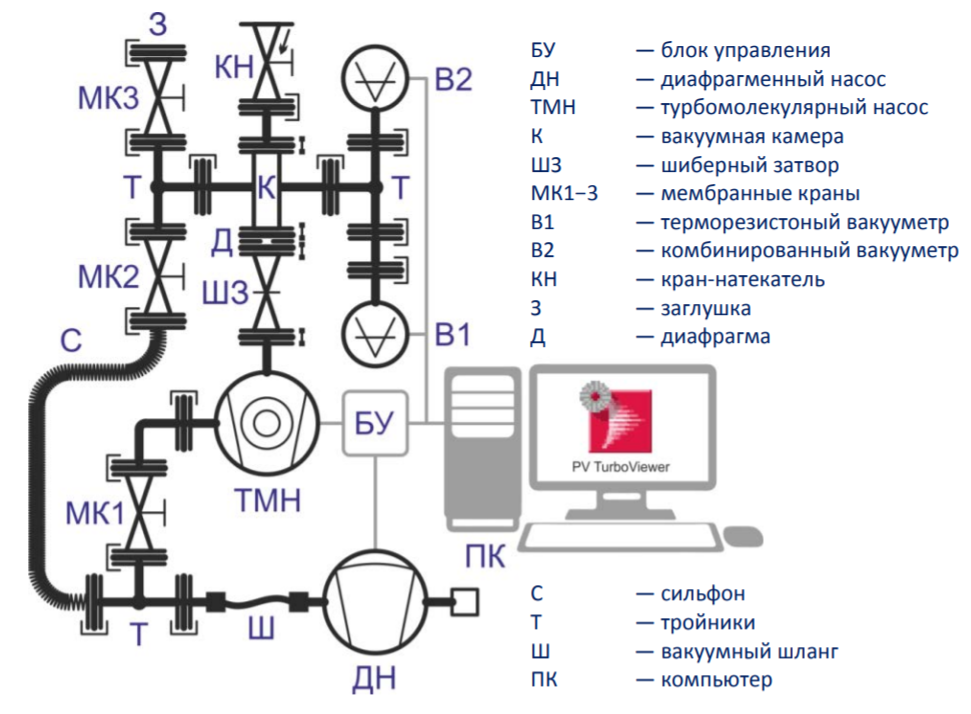
\includegraphics[width = 11.5 cm]{res/Схема}
	\caption{Схема экспериментального стенда}
	\label{fig:vac}
\end{figure}
\begin{figure}[H]
	\centering
	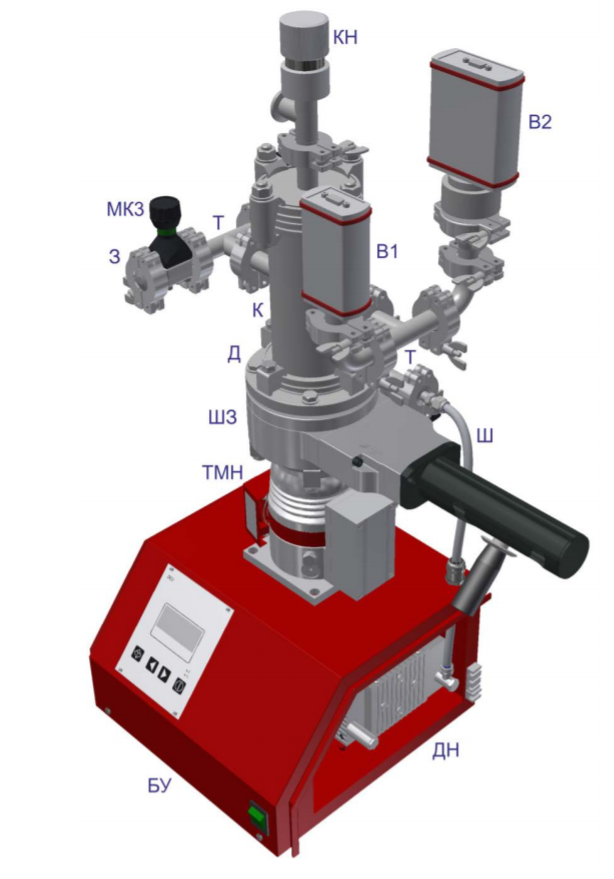
\includegraphics[width = 6.5 cm]{res/Внешний вид}
	\caption{Внешний вид экспериментального стенда}
	\label{fig:vac}
\end{figure}

\begin{figure}[H]
	\caption{Технические характеристики вакууметра В1}
	\label{fig:B1}
	\centering
	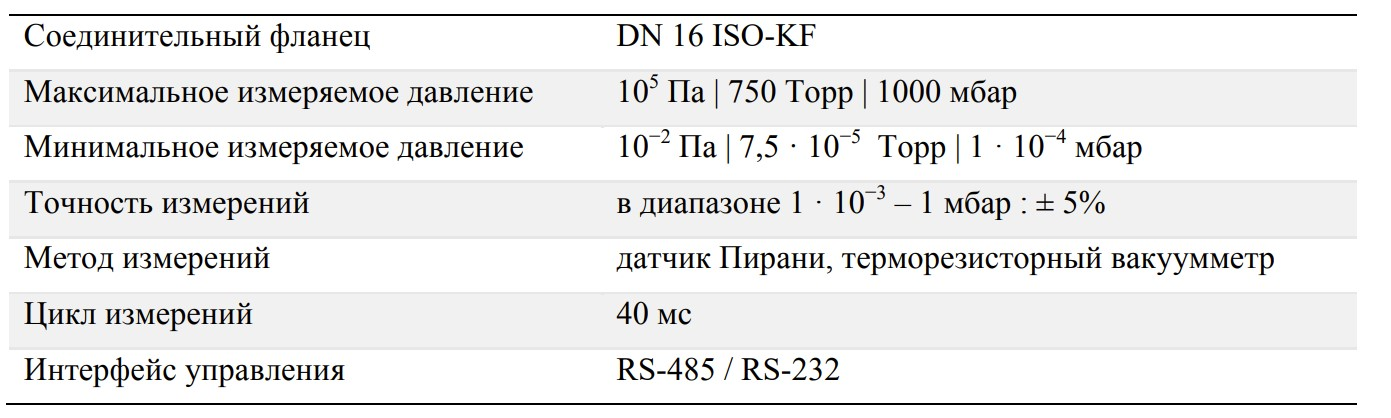
\includegraphics[width = 12 cm]{res/B1технические}
\end{figure}
\begin{figure}[H]
	\caption{Технические характеристики вакууметра В2}
	\label{fig:B2}
	\centering
	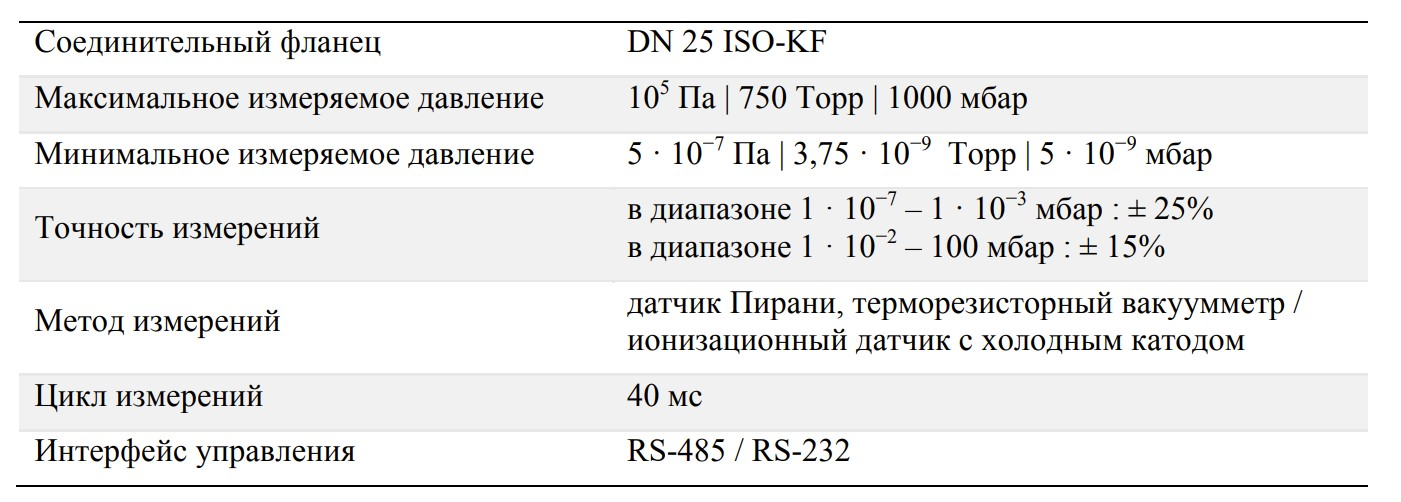
\includegraphics[width = 12 cm]{res/B2технические}
\end{figure}

\subsection*{Ход работы}

\subsubsection*{Определение объемов частей установки}
Присоединяя часть известного объёма к установке, можно измерить давление до и после, из закона Бойля-Мариотта получить сам объём кранов установки.

Для этого проделаем следующее:
\begin{enumerate}
	\item Откачаем установку форвакуумным насосом ДН.
	\item Присоединим к установке сильфон с воздухом при атмосферном давлении.
	\item Выравним давления в сильфоне С и вакуумной камере К экспериментального стенда.
	\item Выравним давление вакуумной камеры К и форвакуумной магистрали установки.
	\item Выравним давление во всей установке, включая объем турбомолекулярного насоса ТМН.
	\item Зафиксируем установившиеся показания вакуумметров.
	
\end{enumerate}

На каждом этапе выравнивания давления фиксируем его. Было проведено 2 измерения, результаты которых занесены в таблицу \ref{tab:press}.

Погрешности определим, используя технические характеристики вакууметра В2 (см. таблицу \ref{fig:B2})



\begin{table}[h]
	\caption{Результаты измерения давления при различных конфигурациях системы}
	\label{tab:press}
	\begin{center}
		\begin{tabular}{lcc}
			\toprule
			{ } & 1 & 2 \\ \midrule
			Действие & $p$, мбар & $p$, мбар  \\ \midrule
			Откачка ДН           & 4.0            & 3,7          	   \\ 
			Открытие МК3         & 220            & 180             \\ 
			Открытие МК2         & 180            & 170             \\ 
			Открытие МК1         & 120            & 120            \\ 
			\bottomrule
		\end{tabular}
	\end{center}
\end{table}


Откуда получаем для объемов следующие значения (см. таблицу \ref{tab:volumes}).
\begin{table}[H]
	\caption{Объемы частей установки}
	\label{tab:volumes}
	\begin{center}
		\begin{tabular}{lc}
			\toprule
			Объем & $(V \pm \sigma_V)$, мл\\ \midrule
			Полной установки           & $1943 \pm 97$  \\ 
			Высоковакуумной части (камера К)         & $1293 \pm 65$ \\ 
			Форвакуумной магистрали         & $649 \pm 32$ \\ 
			\bottomrule
		\end{tabular}
	\end{center}
\end{table}



Теперь проделаем следующее:

\begin{enumerate}
	\item Отсоединим сильфон от установки.
	\item Откачаем установку форвакуумным насосом ДН.
	\item Откачаем объём турбомолекулярным насосом ТМН.
	\item Видно, что терморезисторный вакуумметр $В1$ достиг своего предела измерений, в то время как комбинированный вакуумметр $В2$ (точнее его магнетронная часть) продолжает отображать корректное давление в системе. Зафиксируйте предельное давление в высоковакуумной части установки и время откачки установки насосом ТМН.
	\item Определим уровень течей и скорость откачки системы. Для этого закроем шибер ШЗ, при этом давление в системе начнёт повышаться за счёт наличия течей. Получим таким образом зависимость показаний вакууметра $В2$ от времени. Когда давление превысит $3 \cdot 10^{-3}$ мбар,
	снова откроем шибер. Получим зависимость показаний вакуумметра $В2$ от времени после открытия шибера. Снова зафиксируем предельное давление.
\end{enumerate}

\subsubsection*{Оценка эффективной скорость откачки системы форвакуумным насосом (ДН)}
Мы получили зависимость $p(t)$ при откачке системы ДН. Графики этих зависимостей для разных вакууметров приведены на рисунке \ref{fig:p(t)}. Из графика можно сделать вывод, что для определения постоянной времени откачки следует брать показания вакууметра В1. Строим график $\ln{p}(t)$ (см. рис. \ref{fig:lnB1(t)}) и находим параметры полученной кривой \textbf{методом наименьших квадратов}. Вся статистическая обработка занесена в таблицу \ref{tab:lnB1(t)_stat}.


\begin{figure}[h]
	\centering
		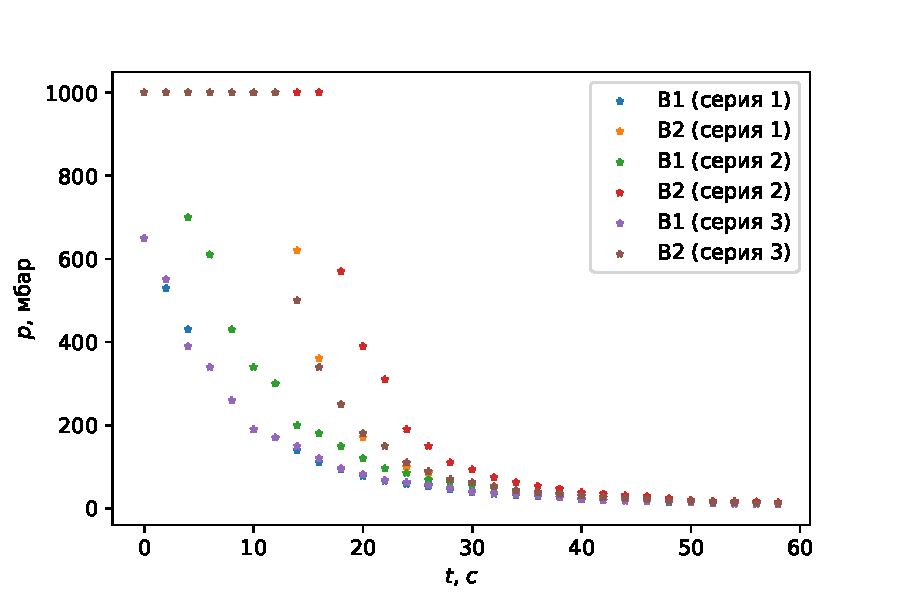
\includegraphics[width = 11 cm]{res/p(t).pdf}
	\caption{График зависимости $p(t)$ ДН}
	\label{fig:p(t)}
\end{figure}

\begin{figure}[H]
	\centering
	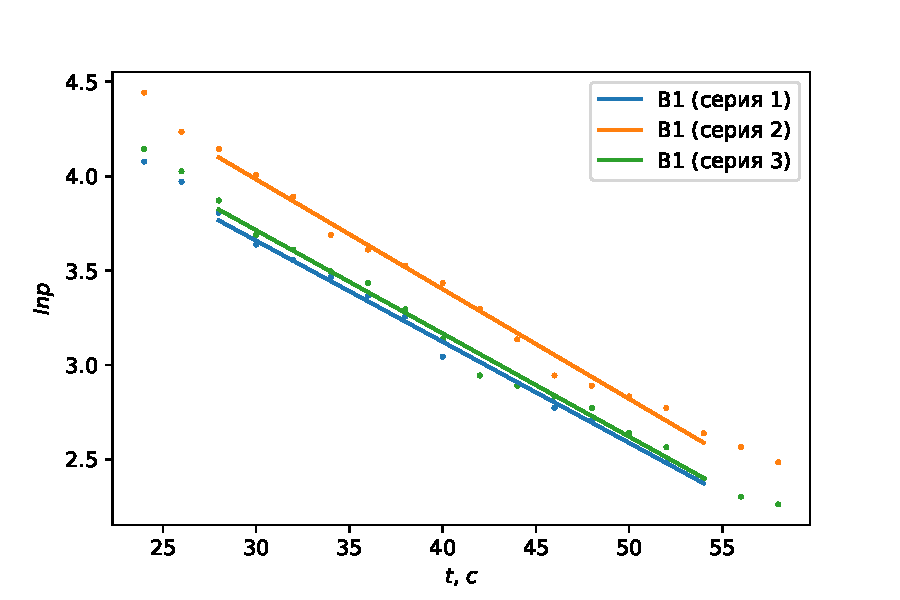
\includegraphics[width = 11 cm]{res/lnB1(t).pdf}
	\caption{График зависимости $\ln{p}(t)$ ДН вакууметра В1}
	\label{fig:lnB1(t)}
\end{figure}
\begin{table}[H]
	
	\caption{Обработка для $Q(P)$}
	\label{tab:lnB1(t)_stat}
	\centering
	\footnotesize
	\begin{tabular}{lccccc}
		\toprule
		
		Серия & $a \pm \sigma_a$ & $b \pm \sigma_b$ \\
		\midrule
		1 & $-0.05354 \pm 0.002720$     &    $5.265 \pm 4.750$ \\ 
		2 & $-0.05813 \pm 0.003382$     &    $5.727 \pm 5.904$ \\
		3 & $-0.05466 \pm 0.003204$     &    $5.354 \pm 5.594$ \\ 
		\bottomrule
	\end{tabular}
\end{table}

Систематическую погрешность оценим, как разность коэффициентов наклона графиков. Полную погрешность - как квадратичную сумму случайной и систематической:
$$	\sigma_{S_0} = \frac{S_0}{a}\sqrt{\sigma_{a}^2 + \Delta a^2} = S_0 \sqrt{0.06^2 + 0.08^2} = 0.1 S_0$$
$$S_0 = -a V_0 = (0.39 \pm 0.04) \frac{\text{л}}{\text{c}}$$

\subsubsection*{Оценка эффективной скорость откачки системы турбомолекулярным (ТМН) насосом}
Аналогичное рассмотрения зависимости $p(t)$ при откачке системы ТМН, а также статистическая обработка результатов приведена на графике \ref{fig:TMHlnB2(t)} и в таблице \ref{tab:TMHlnB2(t)}. 


\begin{figure}[H]
	\caption{График зависимости $\ln{p}(t)$ ТМН вакууметра В2}
	\label{fig:TMHlnB2(t)}
	\centering
	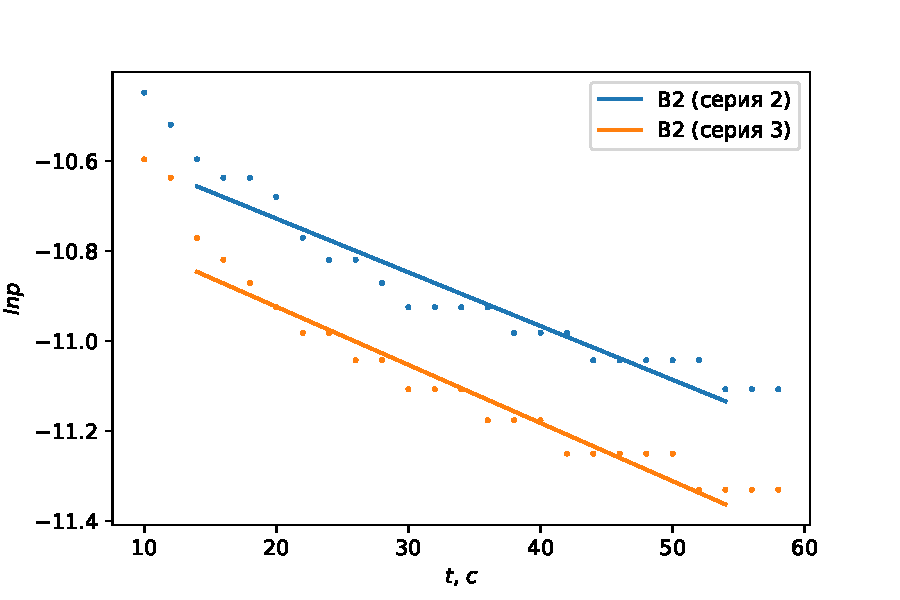
\includegraphics[width = 11 cm]{res/TMHlnB2(t).pdf}
\end{figure}
\begin{table}[H]	
	\caption{Обработка для $Q(P)$}
	\label{tab:TMHlnB2(t)}
	\centering
	\footnotesize
	\begin{tabular}{lccccc}
		\toprule
		
		Серия & $a \pm \sigma_a$ & $b \pm \sigma_b$ \\
		\midrule
		2 & $-0.01194 \pm 0.001593$     &    $-10.49 \pm 2.076$ \\ 
		3 & $-0.01292 \pm 0.001352$     &    $-10.67 \pm 1.762$ \\ 
		\bottomrule
	\end{tabular}
\end{table}

Аналогично систематическую погрешность оценим, как разность коэффициентов наклона графиков. Полную погрешность - как квадратичную сумму случайной и систематической:
$$	\sigma_{S_0} = \frac{S_0}{a}\sqrt{\sigma_{a}^2 + \Delta a^2} = S_0 \sqrt{0.13^2 + 0.08^2} = 0.15 S_0$$
$$S_0 = -a V_k = (0.016 \pm 0.003) \frac{\text{л}}{\text{c}}$$

\subsubsection*{Определение уровня течей по ухудшению вакуума после перекрытия откачки насосом ТМН}
График зависимости $Q_{\text{н}}(t)$ приведен на рисунке \ref{fig:Q(t)}. 
\begin{figure}[H]
	\caption{График зависимости $Q_{\text{н}}(t)$ вакууметра В1}
	\label{fig:Q(t)}
	\centering
	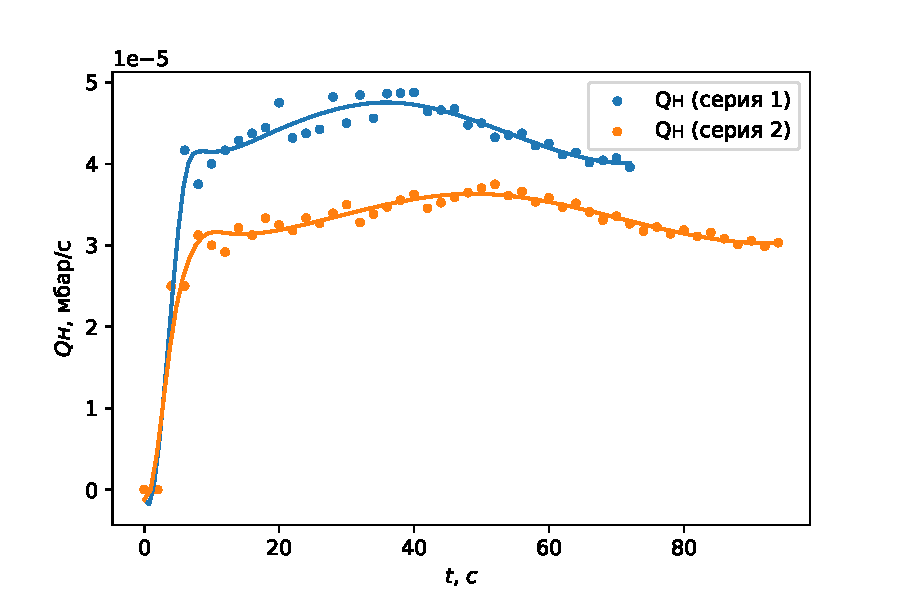
\includegraphics[width = 11 cm]{res/Q(t).pdf}
\end{figure}

Для численной оценки натекания построим график $p(t)$ после перекрытия откачки насосом ТМН.
По угловому коэффициенту определим натекание. Вся статистическая обработка занесена в таблицу \ref{tab:natek}.

\begin{figure}[H]
	\caption{График зависимости $P(t)$ вакууметра В1 после перекрытия откачки насосом ТМН}
	\label{fig:natek}
	\centering
	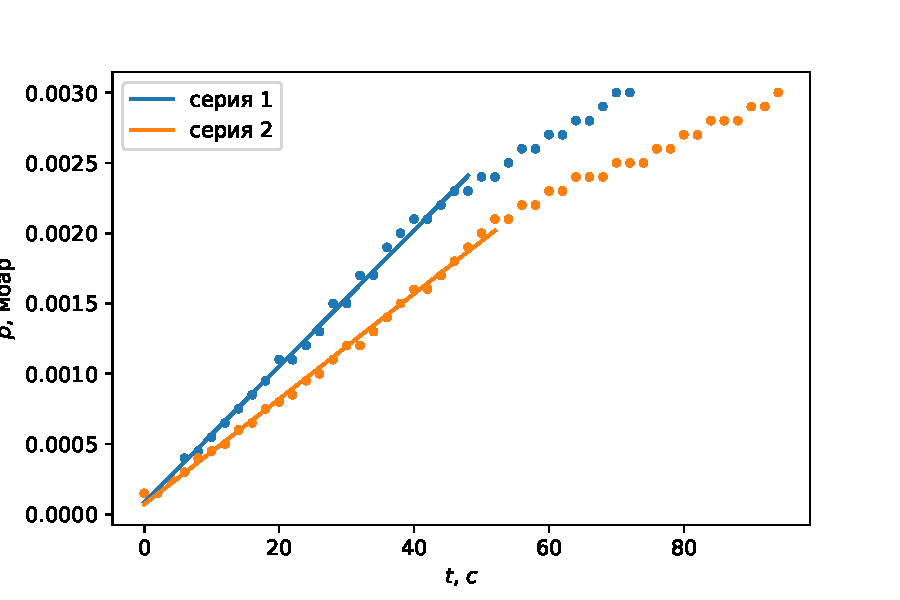
\includegraphics[width = 11 cm]{res/natek.pdf}
\end{figure}

\begin{table}[H]	
	\caption{Обработка зависимости $P(t)$ вакууметра В1 после перекрытия откачки насосом ТМН}
	\label{tab:natek}
	\centering
	\footnotesize
	\begin{tabular}{lccccc}
		\toprule
		
		Серия & $a \pm \sigma_a$ & $b \pm \sigma_b$ \\
		\midrule
		1&$4.842e-05 \pm 1.377e-06$     &    $8.385e-05 \pm 0.001079$  \\
		2&$3.745e-05 \pm 9.298e-07$     &    $7.063e-05 \pm 0.0008542$ \\
		\bottomrule
	\end{tabular}
\end{table}


Откуда получаем величины оценку натекания: 
$$Q_{\text{н}} = (5.5 \pm 0.3)\e{-5}\text{ }\frac{\text{л}\cdot\text{мбар}}{\text{ч}}\ll PS_0$$

\subsection*{Вывод}

Получены вполне правдоподобные результаты. 

Оценка погрешностей была проведена более тщательно, была приведена оценка систематической ошибки. Которую можно оценить, благодаря нескольким сериям одних и тех же измерений.

Эффективная скорость откачки системы форвакуумным насосом достаточно хорошо согласуется с технической характеристикой насоса MVP 015:

$$S_0 = (0.39 \pm 0.04) \frac{\text{м}^3}{\text{ч}}\text{, техн. хар. } 0.50\frac{\text{м}^3}{\text{ч}}$$

Получена оценка эффективной скорость откачки системы турбомолекулярным (ТМН) насосом:
$$S_0 = (0.016 \pm 0.003) \frac{\text{л}}{\text{c}}$$
Также проведен качественный анализ натекания в системе:
$$Q_{\text{н}} = (5.5 \pm 0.3)\e{-5}\text{ }\frac{\text{л}\cdot\text{мбар}}{\text{ч}}\ll PS_0$$


\end{document}